\chapter{Approach}\label{chap:approach}

\section{Problem Definition}
In spite of the fact that JavaScript was originally intended for simple web-pages scripting, it's popularity has increased over the last years, being the most commonly used programming language among professional developers in 2018. Development of robust and high-quality frameworks such as jQuery, AngularJS, React or Vue.js contributed to JavaScript being the leading programming language for client-side development. 

Moreover, several back-end applications are being written in JavaScript using Node.js, thus unifying the programming languages of client and back-end code. Companies with architectures based on concepts such as serverless and microservices are moving traditional back-end code written in Java, Python or PHP to the cloud and replacing it by small compute services, like AWS Lambda or Google Cloud Functions, or directly by cloud managed services. It is very common that development teams decide to write the compute services in Node.js, thus reducing the technological stack.

However, JavaScript was not intented for developing large-scale applications. Lack of good interface descriptions using types and unintuitive type coercion have been slowing development of JavaScript applications.

The TypeScript programming language is a superset of JavaScript with optional type annotations that compiles to plain JavaScript. It has become a widely used alternative for JavaScript. It enables IDEs to perform code intelligence tasks such as code completion, code navigation or refactoring and it rules out possible run-time errors through static type checking.

Aware that types are important for developing maintainable software systems, several industrial developers started using TypeScript in JavaScript projects. However, despite TypeScript's popularity, many new and existing JavaScript Libraries are still being written in pure JavaScript.

The possibility of using exissting JS libraries in TypeScript projects is critical for a smooth transition and for its adoption in industrial development. TypeScript enables it through \textit{declaration files}, a typed description of the library's API. A public repository, DefinitelyTyped \citep{definitely-typed-repository}, contains declaration files for more than 6000 JS Libraries. 71\% of the top 1000 depended-upon packages have their corresponding declaration file in DefinitelyTyped, as explained in \chapref{chap:background}.

Unfortunately, such files are written and maintained manually, which is tedious, error prone and highly time consuming. The evolution of the declaration files does not follow in some cases the continous development of the corresponding libraries. As a result, some declaration files end up being out of date, thus hindering their usability. Mismatches between the declaration files and the actual JavaScript Library code have a negative impact on developers. Type checking messages and IDE code intelligence features are not accurate, thus increasing developing costs, generating actually more difficulties than before migrating to TypeScript.

Declaration files are critical for TypeScript projects. TypeScript's popularity increase and the continuous growth of packages uploaded to the NPM registry, surpassing \textit{1 million} packages by June 2019, indicate that mismatches between declaration files and JavaScript implementations will likely grow. This Thesis tackles the declaration file generation problem and proposes a solution for assiting programmers in creating TypeScript Declaration Files from JavaScript code and keeping them up to date after.

\todo{Agregar una imagen de un modulo simple con codigo JavaScript y que del otro lado salga el declaration file.}

\section{TypeScript Declaration Files Generation Method}

We introduce a \textit{TypeScript Declaration Files Generation Method}, which generates a valid TypeScript Declaration File for a specific JavaScript Library uploaded to the NPM Registry, as explained in \figref{fig:tsd_generation_method_block_diagram}.

\begin{figure}[h]
\begin{centering}
    {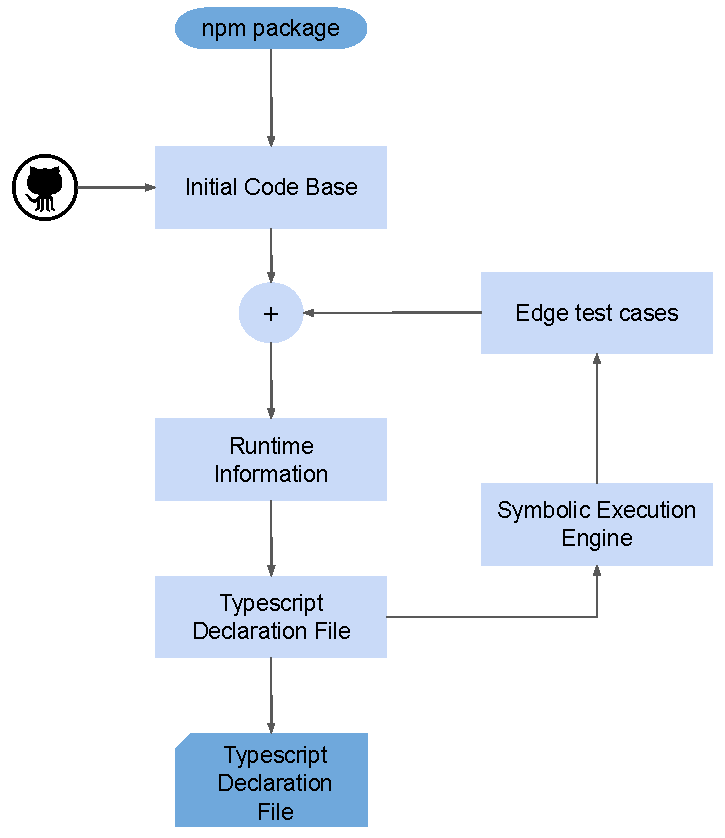
\includegraphics[width=0.9\textwidth]{figures/approach/typescript-declaration-files-generation-method/typescript_declaration_files_generation_method_block_diagram.pdf}}
    \caption[TypeScript Declaration Files Generation Method]{\textbf{TypeScript Declaration Files Generation Method} - Initial code base is retrieved from the npm package's repository. A valid TypeScript Declaration File is generated using run-time information. A Symbolic Execution Engine creates test cases based on the generated Declaration File and via a feedback loop enriches the code base until the stopping criteria is reached. The final TypeScript Declaration File gets returned.}
    \label{fig:tsd_generation_method_block_diagram}
\end{centering}
\end{figure}


The method consists of a continuous refinement process. It generates a TypeScript Declaration File based on data flow and type information gathered at run-time from a code base that executes the JavaScript Library. The code base is expanded by a Symbolic Execution Engine that generates test cases using the generated type definitions. As a result, new execution paths are explored, gathering new run-time information and thus refining the declaration file in every iteration.

Following the goal of easing and automating the generation of TypeScript Declaration Files for existings JavaScript Libraries, the method receives the name of the JavaScript Library published to the NPM Registry as an input argument and returns the corresponding TypeScript declaration file.

The declaration file returned by the method is valid and fully functional, making it suitable for being used within the development process. It contains no errors and matches the structure of the JavaScript Library under analysis, so that the JavaScript code generated after compilation runs. The conducted experiments included tests that consisted on replacing a specific type definition from DefinitelyTyped \citep{definitely-typed-repository} with the one generated in the experiments: TypeScript compilation was sucessful, the generated JavaScript code ran without errors and code intelligence features performed by IDEs like code completion worked as expected.

The feedback loop was not included in the implementation, though. As explained, exploring new execution paths by creating new test cases will refine the declaration files: new types will be assigned to different variables, new interfaces will be detected and existing interfaces will be defined more accurately by detecting new properties. From an incremental point of view, generating the declaration files from run-time information has to be developed in a first place. A declaration file must exist first so that it can be refined afterwards.

For that reason, the decision was to keep the focus on building an end-to-end architecture that supports the generation of valid declaration files for a specific JavaScript Library. The proposed architecture supports a future addition of the refinement loop, without modifying the existing blocks. The Symbolic Execution Engine will expand the existing code base by generating new test cases. The actual generation of declaration files remains unmodified. 

\subsection{Implementation}
As explained before, the DefinitelyTyped Repository is the official repository for finding declaration files for existing JavaScript Libraries. The \textit{TypeScript Declaration Files Generation Method} is intended to be used on existing, published npm packages. The generated output TypeScript declaration file is a valid file which can be used for development and uploaded to the DefinitelyTyped Repository.

Code examples that execute the JavaScript Library are needed to extract the run-time information via code instrumentation. It is achieved by retrieving the examples provided in the README files of the repositories of the different libraries. This is generally the place where developers explicitely show how to use their code. It showed to be an appropriate and pragmatic way of extracting the developer's intention and providing an useful initial code base with meaningful examples, thus avoiding a possible cold start problem. 

The examples and the code base of the library are instrumented with Jalangi \citep{DBLP:conf/sigsoft/SenKBG13}\citep{DBLP:conf/sigsoft/SenKBG13a} to gather data flow information and type information at runtime. Jalangi is a dynamic analysis configurable framework that provides several analysis modules that were extended as needed to retrieve the required run-time information, which is then saved to an output JSON file. This block is written in JavaScript and it runs in Node.js within a Docker container.

A second independent block uses the run-time information to generate a TypeScript Declaration File. It infers the overall structure of the JS Library, the interfaces and the types from the JSON file. This block is a Node.js application written in TypeScript that also runs within a Docker container.

The signatures obtained from the generated declaration file are used to generate pre and post conditions on a Symbolic Execution Engine in order to build different test cases that explore new execution paths. The code from the test cases is then added to the existing code base and the declaration file is generated again using an expanded code base.

Running the TypeScript Declaration File Generation Tool with the same run-time information as input will always produce the same result. If new execution paths are covered by the test cases, new run-time information will be gathered and the declaration file will change accordingly. In order to obtain a sound analysis, the feedback loop would be iterated until the generated declaration files in consecutive iterations do not differ. However, by trading soundness for scalability, the overall procedure can be stopped either using a loop bound, a time bound or an heuristics mechanism.  

\todo{Agregar una imagen mostrando que es un unico script que hace todo. Mostrar imagenes de docker mostrando en qué está escrito cada cosa.}

\section{Initial code base}
To extract run-time information of a JavaScript Library, it is necessary, by definition, to actually execute the code. It is not enough to instrument the source files of the library. The analysis modules provided by Jalangi to gather information are only triggered if the instrumented code gets executed.

We decided to extract the code examples from the Readme files of the repository associated to the NPM Package. Readme files are usually used by developers for briefly describing what the code does, what problem it solves, how to install the application, how to build the code, etc. It is very common that developers provide code examples in the readme files to show how the code works and how to use it. This is specially true for NPM Packages, which are in general created to solve a specific problem of JavaScript development.

Obtaining code examples for a specific NPM Package is achieved in three steps:
\begin{enumerate}
  \item Obtaining the repository from the package.
  \item Retrieving the README file from the repository.
  \item Extract the code examples from the README file.
\end{enumerate}

\subsection{Repository}
The \mintinline{bash}{npm view} command shows data about a package. It is possible to retrieve a specific field of the package registry by specifying fhe field name after the package descriptor. For example to retrieve information about the \textit{lodash} package, the following command can be used: \mintinline{bash}{npm view lodash}.

For this particular case, only the url of the repository associated with the package is needed. This can be achieved by adding the correponding field name: \mintinline{bash}{npm view <PACKAGE> repository.url}.

\begin{bashinline}
$ npm view npm repository.url
git+https://github.com/npm/cli.git

$ npm view lodash repository.url
git+https://github.com/lodash/lodash.git

$ npm view jquery repository.url$
git+https://github.com/jquery/jquery.git
\end{bashinline}

\subsection{Readme files}
The url for downloading a raw file from a Github Repository is the following:

\begin{bashinline}
https://raw.githubusercontent.com/THE-REPOSITORY/master/PATH-TO-FILE
\end{bashinline}

After the repository url is extracted from the npm package, the url for downloading the readme file needs to be constructed performing some string manipulation. Finally, the readme file is obtained with a simple \mintinline{bash}{curl} or \mintinline{bash}{wget} command.

\begin{bashinline}
$ npm view abs repository.url
git+ssh://git@github.com/IonicaBizau/abs.git

$ curl -L -o readme.md --fail \
    https://raw.githubusercontent.com/IonicaBizau/abs/master/README.md
\end{bashinline}

\subsection{Code examples}
Readme files are written using Markdown\footnote{https://www.markdownguide.org}, a very common lightweight and simple markup language. GitHub or BitBucket will convert the readme files into HTML automatically and render them when accessing the repository through a web browser.

It is very common to write code examples within code blocks indicating the programming language, so that it gets highlighted with the specific syntax. The Markdown identifiers for JavaScript are \mintinline{bash}{js} or \mintinline{bash}{javascript}. The code examples are finally retrieved by filtering the content within the corresponding code blocks.

\begin{textinline}
$ cat example-readme.md
# Description
This is an example that shows how to use console.log().

```js
var a = "Hello World!";

function f(s) {
	console.log(s);
}

f(a);
```

$ cat example-readme.md | \
  sed 's/```javascript/```js/g' | \
  sed -n '/^```js/,/^```/ p' > example.js

$ node example.js
Hello World!
\end{textinline}

\section{Run-time Information Gathering} \label{run-time-information-gathering}
As shown in a simple example in \figref{fig:run-time-information-gathering-simple-example}, run-time analysis will gather information such as:

\begin{enumerate}
  \item Function \mintinline{bash}{f} got invoked with parameters \mintinline{bash}{a} and \mintinline{bash}{b} with types \mintinline{bash}{string} and \mintinline{bash}{number}.
  \item Property or method \mintinline{bash}{foo} of parameter \mintinline{bash}{a} of function \mintinline{bash}{f} was accessed within the function.
  \item Parameter \mintinline{bash}{a} of function \mintinline{bash}{f} was used as operand for operator \mintinline{bash}{==}.
\end{enumerate}

The dynamic analysis framework used for gathering this kind of information is Jalangi. As explained in \secref{sec:jalangi}, the configurable analysis modules enable programming custom callbacks that get triggered with virtually any JavaScript event. The events that are observed are:
\begin{enumerate}
  \item Binary operations, like \mintinline{bash}{==}, \mintinline{bash}{+} or \mintinline{bash}{===}.
  \item Variable declaration.
  \item Function, method, or constructor invocation.
  \item Access to an object's property.
  \item Unary operations, like \mintinline{bash}{!} or \mintinline{bash}{typeof}.
\end{enumerate}

The implementation stores these observations as entities called \textit{interactions}. As explained later in \secref{sec:run-time-analysis}, they are used for translating, modifying and aggregating Jalangi's raw event information in order to get an application specific data representation.

The main goal of the run-time analysis is to gather information useful for determining a function's signature. Therefore, observations need to get associated with a function's argument. The implementation wraps variables around Proxy Objects to store tracking data, hereby enabling to associate the observation with a specific argument. The effect is reverted using Jalangi's callbacks to modify the behaviour of the affected operators, such as \mintinline{bash}{===} or \mintinline{bash}{typeof}.

Jalangi fails to instrument some JavaScript Libraries. No effort was made in trying to fix failing instrumentation. Failing JS Libraries were ommited from the analysis by providing a list with the names of the modules that should not be instrumented.

Each function is given an unique key, which is used as the primary key of a map where the run-time information is stored. Each function has an array of arguments and each interaction gets associated with an argument. The map is finally returned as a JSON file that can be used for later processing.

The tool is written in JavaScript and runs in Node.js within a Docker container.

\begin{figure}[tp]
	\centering
	\begin{lrbox}{\mintedbox}
		\begin{minipage}{0.4\textwidth}
			\jscode{code/run-time-information-gathering/simple-examples/simple-example.js}
		\end{minipage}
	\end{lrbox}
	\subfloat[Instrumented JS code]{\usebox{\mintedbox}}
	\hfill
	\begin{lrbox}{\mintedbox}
		\begin{minipage}{0.58\textwidth}
			\jsoncode{code/run-time-information-gathering/simple-examples/output-simple-example.json}
		\end{minipage}
	\end{lrbox}
	\subfloat[Run-time information output]{\usebox{\mintedbox}}
	\caption[Simple run-time information gathering example]{\textbf{Simple run-time information gathering example} - Example code showing \textit{inputValue} and \textit{getField} interactions. Several additional fields and entries of the final output JSON file were omitted for simplicity.}
	\label{fig:run-time-information-gathering-simple-example}
\end{figure}

\subsection{Analysis} \label{sec:run-time-analysis}
The provided analysis module implements the following Jalangi callbacks, which were explained in detail in \secref{sec:jalangi}:
\begin{itemize}
  \item binaryPre()
  \item declare()
  \item getFieldPre()
  \item putFieldPre()
  \item functionEnter()
  \item functionExit()
  \item invokeFun()
  \item invokeFunPre()
  \item unaryPre()
  \item write()
\end{itemize}

They enable observation of all JS operations considered relevant. Every invoked function is given an unique identifier and information for each argument of every function gets stored. The entities \mintinline{bash}{FunctionContainer}, \mintinline{bash}{ArgumentContainer} and \mintinline{bash}{Interaction} are introduced to support the representation of the gathered run-time information. 

Run-time information is stored in a map that contains objects of type \mintinline{bash}{FunctionContainer}.
This entity contains static information about the function as well as implementation specific data needed for generating the right type of declaration file, as explained in \secref{sec:declaration-files-background}. Each field of the entity is explained in \coderef{code:function-container}.

\begin{code}
  \jscode{code/run-time-information-gathering/analysis/function-container.js}
  \caption[FunctionContainer object]{\textbf{\mintinline{bash}{FunctionContainer} object} - \mintinline{bash}{FunctionContainer} is the main entity in the map where the run-time information gets gathered. It contains implementation specific information for the declaration files generation. Entities of type \mintinline{bash}{ArgumentContainer} get appended to the \mintinline{bash}{args} property.}
  \label{code:function-container}
\end{code}

Moreover, as explained in \coderef{code:argument-container}, the \mintinline{bash}{ArgumentContainer} object works as a container for all interactions recorded for that argument. Additionally, it contains simple information about the argument itself, like the index or the name given in the function declaration.

\begin{code}
  \jscode{code/run-time-information-gathering/analysis/argument-container.js}
  \caption[ArgumentContainer object]{\textbf{\mintinline{bash}{ArgumentContainer} object} - The \mintinline{bash}{ArgumentContainer} object works mainly as a container for all relevant observations regarding that argument.}
  \label{code:argument-container}
\end{code}

Finally, observations on the arguments of a function are stored as objects of type \mintinline{bash}{Interaction}. They have to be always associated to an \mintinline{bash}{ArgumentContainer} object or to another \mintinline{bash}{Interaction}. They are explained in detail in \secref{sec:run-time-interactions}.

\subsection{Interactions} \label{sec:run-time-interactions}

\draft{enables the developer to create custom analysis modules by implementing the callbacks to virtually every JavaScript. Jalangi provides a way of writing a custom analysis by implementing}

\subsubsection{\textit{inputValue} interaction}
\begin{figure}[tp]
	\centering
	\begin{lrbox}{\mintedbox}
		\begin{minipage}{0.4\textwidth}
			\jscode{code/run-time-information-gathering/simple-examples/input-value.js}
		\end{minipage}
	\end{lrbox}
	\subfloat[Instrumented JS code]{\usebox{\mintedbox}}
	\hfill
	\begin{lrbox}{\mintedbox}
		\begin{minipage}{0.58\textwidth}
			\jsoncode{code/run-time-information-gathering/simple-examples/output-input-value.json}
		\end{minipage}
	\end{lrbox}
	\subfloat[Run-time information output]{\usebox{\mintedbox}}
	\caption[\textit{inputValue} interaction example]{\textbf{\textit{inputValue} interaction example} - The type of the arguments of function \textit{foo()} is recorded. Several additional fields and entries of the final output JSON file were omitted for simplicity.}
	\label{fig:run-time-information-gathering-input-value}
\end{figure}

\subsubsection{\textit{getField} interaction}
\begin{figure}[tp]
	\centering
	\begin{lrbox}{\mintedbox}
		\begin{minipage}{0.4\textwidth}
			\jscode{code/run-time-information-gathering/simple-examples/get-field.js}
		\end{minipage}
	\end{lrbox}
	\subfloat[Instrumented JS code]{\usebox{\mintedbox}}
	\hfill
	\begin{lrbox}{\mintedbox}
		\begin{minipage}{0.58\textwidth}
			\jsoncode{code/run-time-information-gathering/simple-examples/output-get-field.json}
		\end{minipage}
	\end{lrbox}
	\subfloat[Run-time information output]{\usebox{\mintedbox}}
	\caption[\textit{getField} interaction example]{\textbf{\textit{getField} interaction example} - The accessed properties of argument \textit{a} with their type are recorded. Several additional fields and entries of the final output JSON file were omitted for simplicity.}
	\label{fig:run-time-information-gathering-get-field}
\end{figure}

\subsubsection{\textit{methodCall} interaction}
\begin{figure}[h]
	\centering
	\begin{lrbox}{\mintedbox}
		\begin{minipage}{0.4\textwidth}
			\jscode{code/run-time-information-gathering/simple-examples/method-call.js}
		\end{minipage}
	\end{lrbox}
	\subfloat[Instrumented JS code]{\usebox{\mintedbox}}
	\hfill
	\begin{lrbox}{\mintedbox}
		\begin{minipage}{0.58\textwidth}
			\jsoncode{code/run-time-information-gathering/simple-examples/output-method-call.json}
		\end{minipage}
	\end{lrbox}
	\subfloat[Run-time information output]{\usebox{\mintedbox}}
	\caption[\textit{methodCall} interaction example]{\textbf{\textit{methodCall} interaction example} - The invoked method of argument \textit{a} is recorded. Method information can be accessed through the reference \mintinline{bash}{functionId}, for which, in this example, the \mintinline{bash}{inputValue} interactions are stored. Main entry for \mintinline{bash}{functionId_3} has been ommited. Several additional fields and entries of the final output JSON file were also ommited for simplicity.}
	\label{fig:run-time-information-gathering-method-call}
\end{figure}

\subsubsection{\textit{usedAsArgument} interaction}
\begin{figure}[h]
	\centering
	\begin{lrbox}{\mintedbox}
		\begin{minipage}{0.3\textwidth}
			\jscode{code/run-time-information-gathering/simple-examples/used-as-argument.js}
		\end{minipage}
	\end{lrbox}
	\subfloat[Instrumented JS code]{\usebox{\mintedbox}}
	\hfill
	\begin{lrbox}{\mintedbox}
		\begin{minipage}{0.68\textwidth}
			\jsoncode{code/run-time-information-gathering/simple-examples/output-used-as-argument.json}
		\end{minipage}
	\end{lrbox}
	\subfloat[Run-time information output]{\usebox{\mintedbox}}
	\caption[\textit{usedAsArgument} interaction example]{\textbf{\textit{usedAsArgument} interaction example} - Reporting when an argument is used as an argument of another function provides more accurate information. Several additional fields and entries of the final output JSON file were ommited for simplicity.}
	\label{fig:run-time-information-gathering-used-as-argument}
\end{figure}

\subsubsection{\textit{operator} interaction}

\subsubsection{\textit{followingInteractions}}
\begin{figure}[tp]
	\centering
	\begin{lrbox}{\mintedbox}
		\begin{minipage}{0.4\textwidth}
			\jscode{code/run-time-information-gathering/simple-examples/following-interactions.js}
		\end{minipage}
	\end{lrbox}
	\subfloat[Instrumented JS code]{\usebox{\mintedbox}}
	\hfill
	\begin{lrbox}{\mintedbox}
		\begin{minipage}{0.58\textwidth}
			\jsoncode{code/run-time-information-gathering/simple-examples/output-following-interactions.json}
		\end{minipage}
	\end{lrbox}
	\subfloat[Run-time information output]{\usebox{\mintedbox}}
	\caption[\textit{followingInteractions} interaction example]{\textbf{\textit{followingInteractions} interaction example} - Observations on return values of \mintinline{bash}{getField} and \mintinline{bash}{methodCall} interactions get associated to the leading interaction. Several additional fields and entries of the final output JSON file were omitted for simplicity.}
	\label{fig:run-time-information-gathering-following-interactions}
\end{figure}

\subsubsection{Traces}
\begin{figure}[tp]
	\centering
	\begin{lrbox}{\mintedbox}
		\begin{minipage}{0.46\textwidth}
			\jscode{code/run-time-information-gathering/simple-examples/traces.js}
		\end{minipage}
	\end{lrbox}
	\subfloat[Instrumented JS code]{\usebox{\mintedbox}}
	\hfill
	\begin{lrbox}{\mintedbox}
		\begin{minipage}{0.52\textwidth}
			\jsoncode{code/run-time-information-gathering/simple-examples/output-traces.json}
		\end{minipage}
	\end{lrbox}
	\subfloat[Run-time information output]{\usebox{\mintedbox}}
	\caption[\textit{traces} example]{\textbf{\textit{traces} example} - Interactions on different invocations of a function are stored with different \mintinline{bash}{traces}. Several additional fields and entries of the final output JSON file were omitted for simplicity.}
	\label{fig:run-time-information-gathering-traces}
\end{figure}

\subsection{Wrapper Objects}
\todo{Proxy Objects}
\todo{Primitives}
\todo{Null}
\todo{Undefined}

\subsection{Output Format}
\todo{Explicar que es un JSON con todas las interactions. Explicar estructura de cómo se forma el JSON}


\subsection{Blacklisted Modules}
\begin{figure}[tp]
	\centering
	\begin{lrbox}{\mintedbox}
		\begin{minipage}{0.45\textwidth}
			\jscode{code/blacklisted-modules/foo.js}
		\end{minipage}
	\end{lrbox}
	\subfloat[foo/index.js]{\usebox{\mintedbox}}
	\hfill
	\begin{lrbox}{\mintedbox}
		\begin{minipage}{0.45\textwidth}
			\jscode{code/blacklisted-modules/A.js}
		\end{minipage}
	\end{lrbox}
	\subfloat[A/index.js]{\usebox{\mintedbox}}

	\begin{lrbox}{\mintedbox}
		\begin{minipage}{0.48\textwidth}
			\jscode{code/blacklisted-modules/D.js}
		\end{minipage}
	\end{lrbox}
	\subfloat[D/index.js]{\usebox{\mintedbox}}
	\hfill
	\begin{lrbox}{\mintedbox}
		\begin{minipage}{0.45\textwidth}
			\jsoncode{code/blacklisted-modules/blacklist.json}
		\end{minipage}
	\end{lrbox}
	\subfloat[blacklist.json]{\usebox{\mintedbox}}

	\subfloat{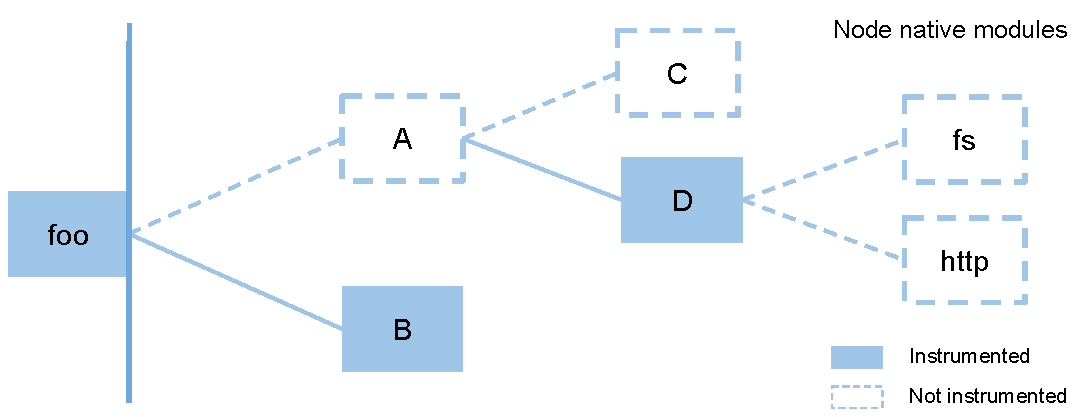
\includegraphics[width=1\textwidth]{figures/approach/blacklisted-modules/blacklisted-modules.pdf}}
	
	\caption[Non-instrumented node modules]{\textbf{Non-instrumented node modules} - Dependencies tree for module \textit{foo}. Modules \textit{A} and \textit{B} are included in the blacklist. Module \textit{D} is instrumented anyway, even though its parent is not. Node native modules, like \textit{fs} or \textit{http}, are excluded anyway by Jalangi.}
	\label{fig:blacklisted-modules}
\end{figure}
\todo{Incluir grafico con los blacklisted modules}

\subsection{Implementation}
\todo{NodeJS \& Docker. Mostrar cómo se invoca, etc.}

\section{TypeScript Declaration File Generation}
\todo{Tres tipos de modulos en TypeScript}
\todo{Traceids y que las signatures de las funciones no se unen, sino que se acumulan segun traceId. Obviamente las iguales no se escriben de vuelta.}
\todo{El nombre de las interfaces se crea con el nombre de la variable}
\todo{El tipo se extrae del valor en runtime.}
\subsection{Implementation}
\todo{TypeScript \& Docker. Mostrar cómo se invoca, etc.}

\section{Evaluation}
\begin{figure}[h]
\begin{centering}
    {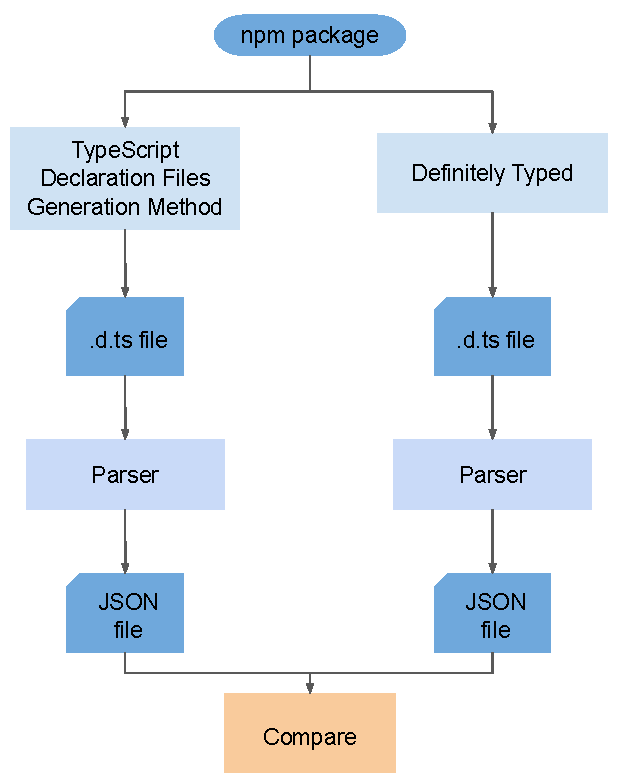
\includegraphics[width=0.8\textwidth]{figures/approach/evaluation/evaluation-diagram.pdf}}
    \caption[Evaluation against DefinitelyTyped Repository]{\textbf{Evaluation of generated declaration files against DefinitelyTyped Repository} - A parser transforms the generated declaration file and the equivalent file in the DefinitelyTyped repository into a JSON file using the TypeScript Compiler API \citep{typescript-compiler-api}. Comparison is then performed on the JSON files, i.e. not on the declaration files.}
    \label{fig:evaluation-diagram}
\end{centering}
\end{figure}

\subsection{Parsing}
\subsubsection{TypeScript Compiler API}
\subsection{Comparison}
\todo{Number of functions}
\todo{Number of parameters}
\todo{Interfaces}
\todo{methodCall}
\todo{usedAsArgument}
\todo{Syntax \& Semantic Errors}